\documentclass[main.tex]{subfiles}

\begin{document}

\hrulefill{}
\subsection{Wave Equation}
Jan 30, 2017

\vspace{3mm}
\subsubsection{Derivation 1}
Wave equation derivation ($u_{tt} - c^2u_{xx} = 0$)

Homework: $u(x, t) = F(x - ct) + G(x + ct)$ is a solution (similar to advection).

Discrete mass-spring system

\begin{figure}[ht]
        \centering
        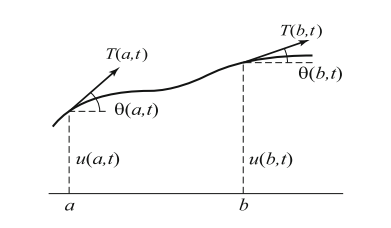
\includegraphics[width=0.5\textwidth]{wave-eq-string}
        \caption{A string with fixed endpoints and $u(x, t)$ representing the vertical displacement of the string.}
        \label{fig:string-wave}
\end{figure}

Let $u(x, t) = \textrm{ the horizontal displacement of the spring from x=0}$

Use Newton's second law:
\begin{align}
F &= mu_{tt}(x, t) \\
  &= \textrm{ left force + right force} \\
  &= k\left[u(x+h, t) - u(x, t)\right] - h \\
  &- k\left[u(x, t) - u(x-h, t) - h\right] \\
  &= kh^2\frac{u(x-h, t) - 2u(x, t) + u(x+h, t)}{h^2} \\
  &= kh^2 u_{xx}
\end{align}

RHS is discrete approximation of $u_{xx}(x, t)$

\begin{align}
f(x) &= f(x) \\
f(x + h) &= f(x) + hf'(x) + h^2\frac{f''(x)}{2} + O(h^3) \\
f(x - h) &= f(x) - hf'(x) + h^2\frac{f''(x)}{2} + O(h^3)
\end{align}
Therefore,

$$-2f(x) + f(x+h) + f(x-h) = f''(x)h^2 + O(h^3)$$

Now take the limit as $h\rightarrow 0+^+$ while scaling $\frac{kh^2}{m} \rightarrow c^2$

Therefore,
\begin{equation}
    u_{tt} = cu_{xx}
\end{equation}

\subsubsection{Derivation 2}

Elastic string/wire
\begin{figure}[ht]
        \centering
        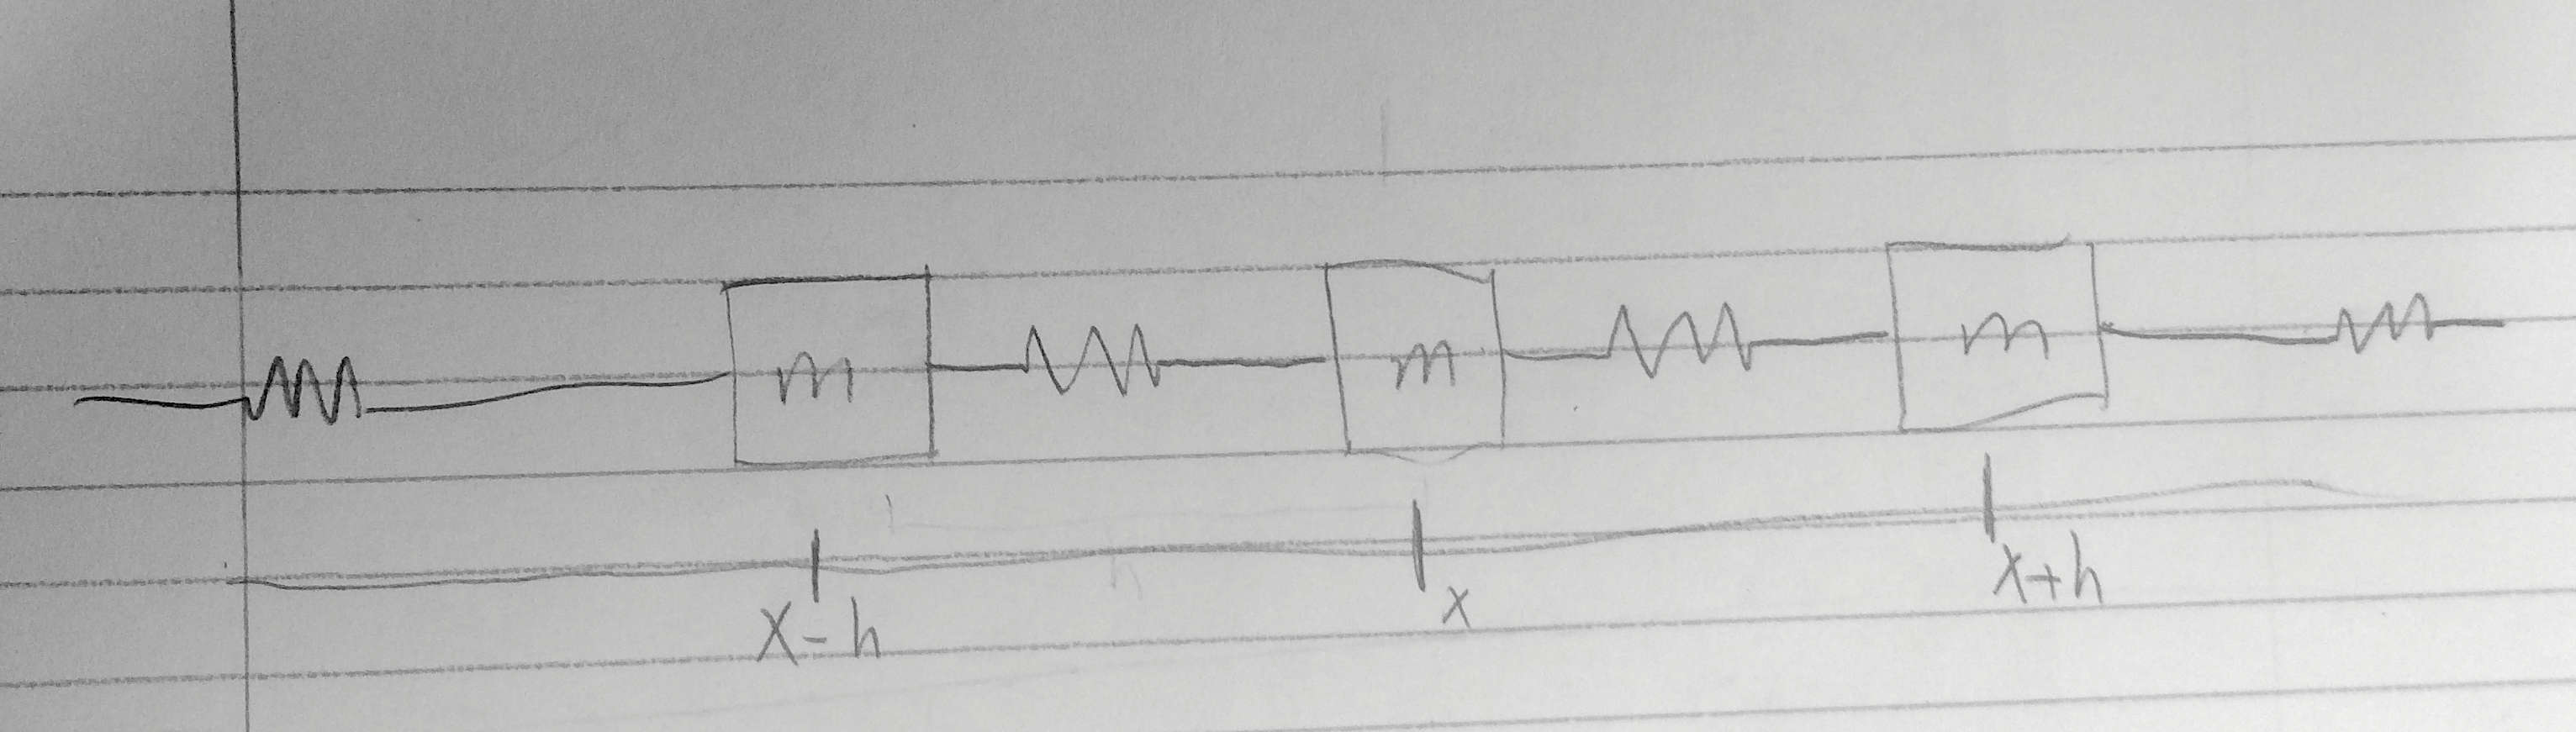
\includegraphics[width=0.7\textwidth]{wave-eq-mass-spring}
        \caption{A system of masses connected with springs, separated by distance $h$ and with mass $m$.}
        \label{fig:discrete-mass-spring-wave}
\end{figure}

Define $u(x, t)$ as vertical displacement of the wire (assuming no horizontal displacement)

Define $T(x, t)$ as tension at $x$ and time $t$, and tangent to the curve.

Resists stretching, not bending.

Define $\rho(x, t)$ as the mass density per length.

Mass balance: $m = \int_a^b \rho(x, t)\sqrt{1+u_x{(x,t)}^2}\,dx = \int_a^b \rho_0(x)$ where $\rho_0$ is the resting or unstretched density.

So, $\forall a, b\implies\rho\sqrt{1+u_x^2} = \rho_0$

Define $\theta(x, t)$ to be the angle by $T(x, t)$ with respect to the horizontal.

No (net) horizontal force:

$T(x, t)\cos{\theta(x, t)}$ = horizontal component of force (independent of $x$) = $\tau(t)$

Change in momentum
$$\int_a^b u_t\rho\sqrt{1+u_x^2}\,dx = \textrm{ total momentum of the segment}$$

Only thing that changes is difference in tensions at endpoints.

\begin{align}
\implies &\frac{d}{dt}\int_a^b u_t\rho\sqrt{1+u_x^2}\,dx \\
         &= T(b, t)\sin{\theta}(b, t) = T(a, t)\sin{\theta(a, t)} \\
         &= T(b, t)\cos{\theta(b, t)}\tan{\theta(b, t)} \\
         &- T(a, t)\cos{\theta(a, t)}\tan{\theta(a, t)}
\end{align}

\begin{align}
\int_a^b u_{tt}\rho_0(x)\,dx &= \tau(t)\left[\tan{\theta(b, t)} - \tan{\theta(a, t)}\right] \\
                             &= \tau(t)\left[u_x(b, t) - u_x(a, t)\right] \\
                             &= \tau(t)\int_a^b u_{xx}\,dx
\end{align}

Therefore,

$$\forall a, b\textrm{, }u_{tt}\rho_0 = \tau u_{xx}$$

Assuming $\tau(t) = \tau_0$ (small displacement, so likely a good approximation), can rewrite as:

$$u_{tt} = {\left(\sqrt{\frac{\tau_0}{\rho_0(x)}}\right)}^2 u_{xx} = c^2 u_{xx}$$

\end{document}
